\section{Fondements théoriques et méthodologiques}

\subsection{Évolution historique et paradigmes d'automatisation}

\subsection{Évolution historique}

La gestion des systèmes d’information a connu une évolution rapide, marquée par plusieurs transformations majeures. Elle est passée de l’administration manuelle des serveurs physiques, où chaque déploiement nécessitait des opérations répétitives et susceptibles d’erreurs, à l’émergence des datacenters virtualisés et du Cloud Computing. Cette progression a été motivée par la recherche d’une meilleure agilité opérationnelle et par la nécessité de réduire les coûts d’exploitation.

La complexification des environnements informatiques a conduit à la formalisation de pratiques visant à automatiser la création, la configuration et la supervision des ressources. C’est dans ce contexte qu’a émergé le paradigme de l’Infrastructure as Code, qui constitue aujourd’hui un socle incontournable des démarches de modernisation.

\subsection{Approche DevOps}

Le développement des infrastructures modernes s’inscrit dans une démarche DevOps, qui associe les équipes de développement et d’exploitation dans une collaboration continue. Cette approche vise à réduire les cycles de livraison, améliorer la qualité logicielle et favoriser l’automatisation des processus. Elle s’appuie sur une culture de responsabilisation partagée, une intégration continue et une surveillance permanente des systèmes. DevOps contribue ainsi à faire converger les objectifs techniques et organisationnels, en alignant la production logicielle et les opérations.

\begin{figure} [H]
	\centering
	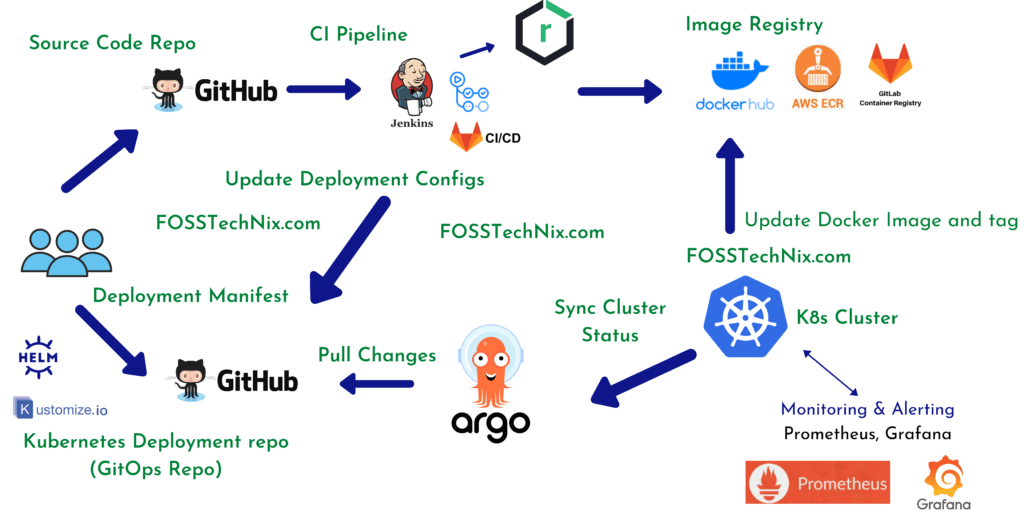
\includegraphics[width=.5\textwidth]{figures/Devops.png}
	\caption{Taches de DevOps}
\end{figure}
\subsection{Modèles conceptuels}

L’Infrastructure as Code (IaC) désigne l’ensemble des méthodes et outils permettant de décrire l’état souhaité d’une infrastructure sous forme de fichiers de configuration versionnés et exécutables. Deux modèles se distinguent généralement : le modèle impératif, dans lequel l’utilisateur décrit la séquence exacte des opérations, et le modèle déclaratif, qui se concentre sur la définition de l’état final visé en laissant au moteur d’exécution la responsabilité d’y converger.

\subsection{Approche GitOps}

En prolongement de l’IaC, l’approche GitOps propose de faire du système de gestion de version la source unique de vérité pour la configuration et le déploiement applicatif. Elle se caractérise par un processus de déploiement automatisé, piloté par des agents qui observent l’état déclaré dans les dépôts et appliquent les modifications nécessaires aux environnements. Cette méthode garantit une traçabilité complète des évolutions, facilite le retour en arrière et renforce la cohérence entre les différents environnements. GitOps s’intègre naturellement avec les pipelines CI/CD, qui orchestrent la construction, les tests et la mise en production de façon systématique.

\section{Conteneurisation et orchestration}

\subsection{Principes de la conteneurisation}

La conteneurisation a constitué une rupture technologique majeure en introduisant une isolation légère des environnements d’exécution, en comparaison avec les machines virtuelles traditionnelles. Chaque conteneur encapsule l’application et ses dépendances, assurant ainsi une portabilité élevée et une reproductibilité des exécutions sur différents environnements.Selon une étude de la CNCF et le rapport State of Containers de Datadog, plus de 80 \% des entreprises utilisant des microservices ont adopté des conteneurs dans leur environnement de production. En 2022, la CNCF rapportait que 42 \% des organisations exécutaient plus de 50 \% de leurs workloads en conteneurs, une proportion qui ne cesse de progresser.Parmi les bénéfices les plus fréquemment identifiés figurent la réduction de la charge système (les conteneurs consomment en moyenne 30 à 50 \% moins de ressources que des machines virtuelles équivalentes), l’optimisation des coûts d’infrastructure, l’accélération des cycles de déploiement (près de 60 \% des entreprises déclarent qu’elles déploient des applications en production plusieurs fois par semaine grâce aux conteneurs) et une meilleure isolation des processus.

\subsection{Orchestration des conteneurs}

Pour coordonner ces conteneurs à grande échelle, des plateformes d’orchestration ont été développées. Kubernetes s’est progressivement imposé comme la solution de référence, grâce à sa capacité à automatiser le placement des workloads, l’ajustement dynamique des ressources, la relance des conteneurs défaillants et la gestion centralisée des configurations ainsi que des secrets.Selon le rapport annuel de la Cloud Native Computing Foundation (CNCF), Kubernetes est aujourd’hui utilisé par plus de 96 \% des organisations qui exploitent des conteneurs en production. Sa popularité ne cesse de croître : en 2016, seuls 27 \% des répondants déclaraient l’utiliser, contre près de 90 \% en 2022, ce qui illustre l’ampleur de son adoption. Ces fonctionnalités favorisent l’exploitation efficace d’environnements complexes et distribués. De plus, plus de 70 \% des entreprises déclarent que Kubernetes joue un rôle stratégique dans leur modernisation applicative et l’adoption du cloud hybride.

\subsection{Patterns d’architecture cloud-native}

La conteneurisation et l’orchestration encouragent l’adoption de modèles applicatifs dits \emph{cloud-native}. Ces architectures reposent notamment sur le découpage en microservices, la scalabilité horizontale, la résilience par la redondance et le découplage entre l’infrastructure et les applications. Ces principes sont aujourd’hui largement adoptés par les entreprises souhaitant moderniser leurs systèmes d’information.

\section{Approches de supervision et d’observabilité}

\subsection{Enjeux de l’observabilité}

Dans des environnements distribués et dynamiques, l’observabilité est un facteur déterminant de fiabilité et de performance. Elle va au-delà de la supervision traditionnelle en visant une compréhension globale et en temps réel des comportements des systèmes. Cette démarche repose sur trois piliers essentiels : les métriques, qui mesurent l’état et les performances ; les logs, qui conservent l’historique des événements ; et les traces distribuées, qui permettent de suivre le parcours des requêtes au sein de l’architecture.

\subsection{Outils et standards de référence}

Différentes solutions se sont imposées comme standards de fait dans le domaine. Prometheus est souvent privilégié pour la collecte des métriques et la génération d’alertes, tandis que Grafana assure leur visualisation et leur suivi en temps réel. Elastic Stack ou Loki sont fréquemment utilisés pour l’agrégation et l’analyse des logs, et des outils tels que Jaeger et OpenTelemetry facilitent le traçage distribué. L’adoption de protocoles ouverts et d’API standardisées favorise leur intégration avec les plateformes d’orchestration.

\section{Sécurité des infrastructures automatisées}

\subsection{Principes de sécurité}

La sécurisation des infrastructures automatisées s’appuie sur le principe de \emph{Security by Design}, qui préconise l’intégration des mesures de protection dès les phases initiales de conception. Le modèle \emph{Zero Trust}, largement diffusé, repose notamment sur l’absence de confiance implicite accordée à un composant, l'identification, l’authentification et l’autorisation systématiques de chaque requête ainsi que la limitation des privilèges au strict nécessaire. Ces approches sont particulièrement adaptées aux environnements hybrides et multi-clouds.

\subsection{Gestion des secrets et des accès}

La gestion centralisée des secrets constitue une pratique essentielle pour sécuriser les identifiants, certificats et autres éléments sensibles. Elle repose sur le stockage chiffré, la rotation périodique des clés et la traçabilité des accès. Des outils spécialisés, tels que Vault, apportent des solutions robustes et éprouvées pour répondre à ces exigences.

\subsection{Sécurité périmétrique et segmentation}

La protection des infrastructures repose également sur des dispositifs périmétriques tels que les pare-feu, les listes de contrôle d’accès et la segmentation réseau. Ces mécanismes permettent de limiter la surface d’exposition, de cloisonner les environnements et de renforcer la résilience face aux attaques latérales. La mise en œuvre de politiques de filtrage strictes et le principe du moindre privilège complètent ces mesures pour réduire les risques d’intrusion.

\subsection{Option : pfSense en tant que routeur et pare-feu principal}

Dans l’architecture retenue, il est possible de déployer pfSense comme machine virtuelle dédiée assurant le rôle de passerelle unique et de point de contrôle des flux réseau. Dans ce scénario, pfSense est connecté à deux interfaces réseau distinctes :

\begin{itemize}
	\item Une interface \textbf{LAN}, reliée au réseau interne Proxmox et aux machines virtuelles.
	\item Une interface \textbf{WAN}, reliée au réseau externe (Internet).
\end{itemize}

Toutes les machines virtuelles définissent pfSense comme leur passerelle par défaut. Cela permet :

\begin{itemize}
	\item De centraliser le filtrage et le NAT.
	\item De contrôler et journaliser l’ensemble des flux entrants et sortants.
	\item D’appliquer des politiques de segmentation et de routage spécifiques par VLAN ou sous-réseau.
	\item D’établir des tunnels VPN (IPSec, OpenVPN) de manière centralisée.
\end{itemize}

Cette approche offre une séparation claire entre le plan de gestion (Proxmox) et le plan de données (trafic applicatif), améliorant la sécurité globale.

\begin{figure}[H]
	\centering
	\begin{tikzpicture}[
			node distance=2cm,
			box/.style={draw, rectangle, minimum width=3cm, minimum height=1cm, align=center},
			vm/.style={draw, rectangle, minimum width=2cm, minimum height=0.8cm, align=center}
		]
		% Nodes
		\node[box] (internet) {Internet};
		\node[box, below of=internet] (proxmox) {Proxmox Hyperviseur};
		\node[box, below of=proxmox] (pfsense) {VM pfSense \\ (Pare-feu / Routeur)};
		\node[box, below of=pfsense] (switch) {Réseau LAN Interne};
		\node[vm, left=1.5cm of switch] (vm1) {VM1};
		\node[vm, right=1.5cm of switch] (vm2) {VM2};
		% Arrows
		\draw[->] (internet) -- (proxmox);
		\draw[->] (proxmox) -- (pfsense);
		\draw[->] (pfsense) -- (switch);
		\draw[->] (switch) -- (vm1);
		\draw[->] (switch) -- (vm2);
	\end{tikzpicture}
	\caption{Architecture avec pfSense en tant que routeur et pare-feu principal}
\end{figure}

Cette configuration permet de garantir que tout le trafic réseau transite par pfSense, offrant un contrôle périmétrique complet et la possibilité d’appliquer des politiques de sécurité avancées.

\subsection{Réplication et résilience}

La réplication et la résilience constituent des aspects essentiels de l’infrastructure mise en place, afin de garantir la haute disponibilité des services et la continuité des opérations en cas d’incident.

\paragraph{Virtualisation et clustering Proxmox}
Au niveau de la virtualisation, un cluster Proxmox a été configuré avec plusieurs nœuds physiques interconnectés, permettant de mutualiser les ressources et de répartir les charges de travail. Plusieurs approches existent pour assurer la continuité de service en cas de défaillance matérielle :

\begin{itemize}
	\item \textbf{Réplication manuelle des machines virtuelles}, qui consiste à effectuer périodiquement des copies complètes des disques virtuels sur un autre hôte. Cette approche présente l’avantage d’être simple à mettre en place, mais elle implique des délais de récupération plus longs, car il faut importer et redémarrer la VM sur un autre nœud après une panne.
	\item \textbf{Réplication programmée via Proxmox}, qui offre la possibilité de définir des règles de réplication asynchrone (par exemple toutes les 15 minutes) vers un nœud cible. En cas d’incident, la VM peut être démarrée rapidement sur l’hôte de secours à partir du dernier état synchronisé. Cette approche réduit considérablement le RTO (Recovery Time Objective), tout en restant plus simple à opérer que des solutions de stockage distribuées.
	\item \textbf{Stockage distribué Ceph}, qui permet de disposer d’un volume partagé entre tous les nœuds du cluster, avec réplication synchrone des données et tolérance aux pannes disque et hôte. Cette solution est plus complexe à déployer et nécessite un minimum de trois nœuds, mais elle offre un haut niveau de résilience et la possibilité de migrer dynamiquement les VM sans interruption.
\end{itemize}

Le cluster en place privilégie une approche combinant la réplication programmée pour les VM critiques et un stockage partagé Ceph pour les ressources nécessitant un très haut niveau de disponibilité.

\paragraph{Sauvegarde des données}
La sauvegarde des données est assurée par Proxmox Backup Server, qui permet d’effectuer des sauvegardes incrémentielles planifiées et chiffrées des machines virtuelles et des conteneurs. Contrairement à une simple réplication, la sauvegarde conserve un historique versionné, facilitant la restauration en cas de corruption de données ou d’erreur humaine. Les sauvegardes sont stockées sur un volume dédié, avec vérification d’intégrité et possibilités de restauration granulaire.

\paragraph{Stockage persistant dans Kubernetes}
En complément de la virtualisation, le stockage des volumes persistants dans l’environnement Kubernetes repose sur Longhorn. Plusieurs options étaient envisageables :
\begin{itemize}
	\item L’utilisation de volumes locaux, plus performants, mais ne permettant pas de réplication automatique entre les nœuds.
	\item Le recours à un stockage NFS externe, qui simplifie la mutualisation mais peut devenir un point unique de défaillance.
	\item L’intégration de solutions distribuées comme Rook-Ceph ou Longhorn, permettant la réplication synchrone des volumes, les snapshots, et la tolérance aux pannes.
\end{itemize}
Longhorn a été retenu pour sa simplicité de mise en œuvre et sa capacité à assurer la résilience des volumes persistants sans dépendance externe, en maintenant automatiquement plusieurs répliques synchronisées sur des nœuds distincts.

\paragraph{Réseau et accès externe}
L’accès aux services exposés à Internet est assuré par un reverse proxy. Plusieurs stratégies sont envisageables :
\begin{itemize}
	\item Héberger le reverse proxy directement sur un des nœuds Proxmox, ce qui simplifie l’architecture mais implique un couplage entre l’hyperviseur et le point d’entrée réseau.
	\item Déployer le reverse proxy dans un cluster Kubernetes, avec des réplicas et des LoadBalancers qui répartissent les connexions.
	\item Séparer le reverse proxy sur des VMs dédiées (ou des serveurs physiques distincts), avec une configuration VRRP (via Keepalived) pour disposer d’une IP virtuelle flottante. En cas de panne d’un nœud, l’IP est automatiquement reprise par l’instance survivante, assurant une continuité de service transparente.
\end{itemize}
Dans l’architecture retenue, le reverse proxy est externalisé sur des VMs dédiées, configurées en haute disponibilité avec Keepalived. Cette séparation garantit que la couche de routage HTTP et HTTPS n’est pas dépendante de l’état des hyperviseurs.

\paragraph{Réplication et résilience applicative}
Concernant les applications elles-mêmes, le cluster Kubernetes est configuré pour exécuter plusieurs réplicas des pods assurant les services critiques. Les déploiements définissent un nombre minimal de réplicas répartis sur des nœuds distincts. Ainsi, la perte d’un hôte n’interrompt pas la disponibilité du service. Les probes de liveness et readiness assurent la surveillance de la santé des instances, permettant leur redémarrage automatique en cas de défaillance logicielle. L’autoscaling horizontal complète le dispositif en ajustant dynamiquement le nombre de réplicas selon la charge.

\paragraph{Comparaison synthétique des approches}
\begin{table}[H]
	\renewcommand{\arraystretch}{1.3}
	\centering
	\begin{tabular}{|p{4cm}|p{5cm}|p{5cm}|}
		\hline
		\textbf{Aspect}                 & \textbf{Approche minimale}               & \textbf{Approche avancée (retenue)}                   \\
		\hline
		Stockage VM                     & Disques locaux avec réplication manuelle & Ceph distribué avec réplication synchrone             \\
		\hline
		Sauvegardes                     & Copie manuelle périodique                & Proxmox Backup Server avec incrémental et chiffrement \\
		\hline
		Reverse proxy                   & Service unique sur un hyperviseur        & VMs dédiées + Keepalived avec IP flottante            \\
		\hline
		Volumes Kubernetes              & Volumes locaux/NFS simple                & Longhorn avec répliques synchrones et snapshots       \\
		\hline
		Haute disponibilité VMs         & Migration manuelle après panne           & HA Proxmox avec redémarrage automatique               \\
		\hline
		Haute disponibilité applicative & Un seul pod sans réplication             & Réplicas multiples et autoscaling                     \\
		\hline
	\end{tabular}
	\caption{Comparaison des options de réplication et résilience}
\end{table}

L’ensemble de ces mesures contribue à renforcer la tolérance aux pannes de l’infrastructure, en combinant la redondance au niveau des ressources physiques, la réplication des données et la résilience logicielle des applications.

\subsection{Distribution du réseau}

La distribution du réseau constitue un fondement essentiel de l’architecture moderne, permettant d’assurer la scalabilité, la tolérance aux pannes et la performance des services.

\paragraph{Segmentation et isolation}
Afin de garantir la sécurité et l’isolation des flux, l’infrastructure est segmentée en plusieurs sous-réseaux virtuels (VLAN) :
\begin{itemize}
	\item Un réseau interne réservé aux communications entre hyperviseurs et au trafic de stockage distribué.
	\item Un réseau de management, isolé des services applicatifs, pour l’administration sécurisée des nœuds.
	\item Un réseau applicatif sur lequel sont exposés les pods Kubernetes et les services internes.
	\item Un réseau public dédié à la publication des applications via le reverse proxy.
\end{itemize}
Cette séparation limite la surface d’attaque et réduit le risque de propagation d’incident.

\paragraph{Haute disponibilité et équilibrage de charge}
Plusieurs stratégies existent pour distribuer le trafic :
\begin{itemize}
	\item \textbf{Approche monolithique}, reposant sur un seul point d’entrée réseau (reverse proxy unique), plus simple mais vulnérable en cas de défaillance.
	\item \textbf{Approche active-passive} avec VRRP (Keepalived), qui met en place une IP flottante basculant automatiquement entre deux nœuds en cas de panne.
	\item \textbf{Approche active-active}, consistant à disposer de plusieurs points d’entrée en équilibrage de charge, avec synchronisation des configurations (par exemple HAProxy + Consul Template). Cette approche offre une scalabilité horizontale et une meilleure tolérance aux pannes.
\end{itemize}
L’infrastructure mise en place adopte une combinaison d’un cluster de reverse proxies déployés sur des VMs dédiées et d’un mécanisme VRRP assurant la continuité de l’adresse IP publique.

\paragraph{Routage interne et service discovery}
Les communications entre microservices dans Kubernetes sont gérées via le DNS interne CoreDNS, qui résout automatiquement les noms des services et assure la découverte dynamique. Pour certaines applications nécessitant une tolérance accrue, un service mesh (comme Istio ou Linkerd) peut être ajouté afin d’enrichir le routage, la sécurité mutuelle (mTLS) et la résilience (circuit breaking).

\paragraph{Comparaison des approches}
\begin{table}[H]
	\renewcommand{\arraystretch}{1.3}
	\centering
	\begin{tabular}{|p{4cm}|p{5cm}|p{5cm}|}
		\hline
		\textbf{Aspect}        & \textbf{Approche simple} & \textbf{Approche distribuée avancée} \\
		\hline
		Points d’entrée réseau & Reverse proxy unique     & Plusieurs reverse proxies actifs     \\
		\hline
		Haute disponibilité IP & Non, dépend du nœud      & VRRP avec IP flottante               \\
		\hline
		Service discovery      & Résolution DNS simple    & Service mesh avec routage avancé     \\
		\hline
		Isolation des flux     & VLAN minimal             & Segmentation stricte par rôle        \\
		\hline
	\end{tabular}
	\caption{Comparaison des stratégies de distribution réseau}
\end{table}

L’ensemble de cette configuration permet d’assurer un routage robuste et un point d’entrée tolérant aux pannes pour l’ensemble des services.

\subsection{Distribution du traitement}

La distribution du traitement vise à découpler l’exécution des charges de travail sur plusieurs ressources matérielles et logicielles, afin d’optimiser la disponibilité et la scalabilité.

\paragraph{Virtualisation et orchestration}
Le cluster Proxmox offre la première couche de distribution, en permettant de répartir les VM et conteneurs sur plusieurs hyperviseurs. Les ressources CPU et mémoire peuvent être ajustées dynamiquement par migration des charges (Live Migration), ce qui autorise des opérations de maintenance sans interruption.

Au-dessus de cette couche, Kubernetes orchestre les applications conteneurisées en multipliant les réplicas des pods sur les nœuds disponibles. Chaque déploiement spécifie :
\begin{itemize}
	\item Le nombre minimal et maximal de réplicas.
	\item Les contraintes d’affinité (anti-affinity) garantissant leur répartition sur différents hôtes physiques.
	\item Les ressources CPU/mémoire réservées et limites pour chaque pod.
\end{itemize}
Cette stratégie permet d’assurer la continuité du service même lors de la perte d’un nœud.

\paragraph{Autoscaling et gestion de la charge}
Plusieurs mécanismes de scaling sont mis en place :
\begin{itemize}
	\item \textbf{Horizontal Pod Autoscaler (HPA)} qui ajuste dynamiquement le nombre de réplicas en fonction de la consommation CPU ou des métriques personnalisées.
	\item \textbf{Vertical Pod Autoscaler (VPA)} qui ajuste automatiquement les ressources allouées à chaque pod.
	\item \textbf{Cluster Autoscaler}, qui peut provisionner de nouveaux nœuds si la capacité devient insuffisante.
\end{itemize}
Dans un contexte haute disponibilité, ces fonctionnalités garantissent une adaptation continue à la charge, tout en conservant une redondance suffisante.

\paragraph{Comparaison des stratégies de traitement}
\begin{table}[H]
	\renewcommand{\arraystretch}{1.3}
	\centering
	\begin{tabular}{|p{4cm}|p{5cm}|p{5cm}|}
		\hline
		\textbf{Aspect}         & \textbf{Approche statique}      & \textbf{Approche dynamique distribuée}              \\
		\hline
		Placement des workloads & Affectation fixe sur un hôte    & Orchestration dynamique par Kubernetes              \\
		\hline
		Scalabilité             & Manuelle                        & Autoscaling horizontal et vertical                  \\
		\hline
		Disponibilité           & Réplication minimale ou absente & Réplicas multiples avec anti-affinité               \\
		\hline
		Maintenance             & Arrêt manuel des VM             & Migration transparente et redéploiement automatique \\
		\hline
	\end{tabular}
	\caption{Comparaison des approches de distribution du traitement}
\end{table}

Cette distribution automatisée du traitement garantit une meilleure résilience face aux pannes et une adaptation continue à la demande.

\subsection{Distribution du stockage}

La distribution du stockage vise à assurer la durabilité, la performance et la disponibilité des données, en s’appuyant sur des mécanismes de réplication et de tolérance aux pannes.

\paragraph{Stockage des disques virtuels}
Pour les machines virtuelles, plusieurs options ont été étudiées :
\begin{itemize}
	\item \textbf{Stockage local} : chaque hôte stocke les disques sur un volume interne (SSD ou HDD). Simple à configurer, cette approche présente un risque élevé de perte en cas de panne.
	\item \textbf{Stockage NFS partagé} : un serveur central héberge les disques. Ce modèle simplifie le partage mais devient un point unique de défaillance.
	\item \textbf{Stockage Ceph distribué} : tous les nœuds participent au stockage, avec réplication automatique des blocs et rebalancing dynamique en cas de panne d’un disque ou d’un hôte.
\end{itemize}
L’architecture privilégie Ceph, qui offre un bon compromis entre performance, redondance et évolutivité.

\paragraph{Stockage des volumes Kubernetes}
Pour les applications conteneurisées, Longhorn a été choisi :
\begin{itemize}
	\item Chaque volume est répliqué en temps réel sur plusieurs nœuds.
	\item Les snapshots incrémentaux permettent des restaurations rapides.
	\item Le système de scheduling des réplicas garantit leur distribution sur des hôtes distincts.
\end{itemize}
Cette approche élimine les points de défaillance uniques et simplifie la gestion des volumes persistants.

\paragraph{Sauvegarde et archivage}
La sauvegarde des données est assurée par un système multi-niveaux :
\begin{itemize}
	\item \textbf{Snapshots Ceph et Longhorn}, pour des points de restauration rapides.
	\item \textbf{Sauvegardes incrémentielles chiffrées via Proxmox Backup Server}, permettant un stockage historique et une restauration granulaire.
	\item \textbf{Archivage distant}, avec synchronisation vers un dépôt externe pour protéger contre les sinistres majeurs.
\end{itemize}

\paragraph{Comparaison des approches de stockage}
\begin{table}[H]
	\renewcommand{\arraystretch}{1.3}
	\centering
	\begin{tabular}{|p{4cm}|p{5cm}|p{5cm}|}
		\hline
		\textbf{Aspect}      & \textbf{Approche locale}              & \textbf{Approche distribuée}                     \\
		\hline
		Redondance           & Aucune                                & Réplication synchrone multi-nœuds                \\
		\hline
		Performance          & Locale, rapide                        & Équilibrée selon le réseau et les disques        \\
		\hline
		Tolérance aux pannes & Perte de données si panne disque/nœud & Données conservées malgré plusieurs défaillances \\
		\hline
		Scalabilité          & Capacité limitée par hôte             & Extension linéaire en ajoutant des nœuds         \\
		\hline
	\end{tabular}
	\caption{Comparaison des options de distribution du stockage}
\end{table}

Ces mécanismes contribuent à garantir la sécurité et la continuité des données, en limitant les impacts des défaillances matérielles et logicielles.

\subsection{Sauvegarde et restauration}

La sauvegarde et la restauration des données constituent un pilier central de la stratégie de continuité d’activité. Elles complètent les mécanismes de haute disponibilité et de réplication, en permettant de récupérer des données perdues ou corrompues, y compris en cas d’incidents majeurs (pannes simultanées, erreurs humaines, attaques).

\paragraph{Objectifs et distinction avec la haute disponibilité}
La sauvegarde diffère fondamentalement de la haute disponibilité :
\begin{itemize}
	\item La \textbf{haute disponibilité} (HA) vise à garantir que le service continue de fonctionner sans interruption notable, même en cas de défaillance matérielle ou logicielle, grâce à la redondance et au basculement automatique.
	\item La \textbf{sauvegarde} (backup) vise à conserver une copie historisée des données à un instant donné, indépendamment du fonctionnement du système. Elle permet de revenir en arrière après une corruption, une suppression accidentelle ou une compromission.
\end{itemize}
Ainsi, la haute disponibilité n’élimine pas la nécessité de disposer de sauvegardes fiables : un système HA peut propager une erreur ou une suppression sur tous les nœuds.

\paragraph{Snapshots vs. sauvegardes}
Il est également essentiel de distinguer les \textbf{snapshots} des sauvegardes classiques :
\begin{itemize}
	\item Un \textbf{snapshot} est une image instantanée d’un volume ou d’une machine virtuelle, généralement stockée sur le même système que les données originales. Il permet une restauration rapide mais ne protège pas contre une perte physique du support.
	\item Une \textbf{sauvegarde} est exportée et stockée sur un système séparé, parfois chiffré et versionné. Elle répond au principe fondamental de la règle «3-2-1» (3 copies, sur 2 supports différents, dont 1 hors site).
\end{itemize}
Dans l’infrastructure mise en place, les snapshots Ceph ou Longhorn sont utilisés pour des restaurations rapides, tandis que les sauvegardes incrémentielles Proxmox Backup Server assurent une protection durable et hors site.

\paragraph{Types de sauvegardes}
Plusieurs stratégies de sauvegarde coexistent :

\begin{itemize}
	\item \textbf{Sauvegarde complète} : copie intégrale de toutes les données à chaque exécution. Elle simplifie la restauration mais consomme un espace disque important et augmente la durée des sauvegardes.
	\item \textbf{Sauvegarde différentielle} : copie uniquement les modifications apportées depuis la dernière sauvegarde complète. Lors de la restauration, il suffit de combiner la sauvegarde complète et la dernière différentielle.
	\item \textbf{Sauvegarde incrémentielle} : copie les modifications depuis la dernière sauvegarde (complète ou incrémentielle). Elle minimise l’espace requis et la durée de l’opération, mais la restauration nécessite de rejouer la chaîne complète d’incréments.
\end{itemize}
Proxmox Backup Server repose sur une approche incrémentielle optimisée par déduplication et vérification d’intégrité, offrant un bon compromis entre rapidité et sécurité.

\paragraph{Sauvegarde des machines virtuelles}
Les VM Proxmox sont sauvegardées selon une politique planifiée :
\begin{itemize}
	\item Sauvegarde complète hebdomadaire.
	\item Sauvegarde incrémentielle quotidienne.
	\item Rétention configurée pour conserver plusieurs versions et éviter la saturation du stockage.
\end{itemize}
Chaque sauvegarde est chiffrée, signée et vérifiée par Proxmox Backup Server. Cette granularité permet de restaurer une VM entière ou des fichiers spécifiques.

\paragraph{Sauvegarde des volumes persistants Kubernetes}
Pour Kubernetes, Longhorn offre une gestion avancée des snapshots et sauvegardes :
\begin{itemize}
	\item Les \textbf{snapshots} permettent de capturer un état instantané du volume et de le restaurer localement.
	\item Les \textbf{sauvegardes} Longhorn sont exportées vers un stockage objet (MinIO ou S3), garantissant leur conservation hors du cluster.
\end{itemize}
Ces sauvegardes sont déclenchées automatiquement après certaines opérations critiques et complétées par des sauvegardes applicatives (par exemple, dumps de base de données).

\paragraph{Archivage distant}
Un mécanisme d’archivage complémentaire synchronise périodiquement les sauvegardes vers un dépôt externe géographiquement séparé. Cette mesure protège contre les sinistres majeurs tels qu’un incendie ou un ransomware affectant l’infrastructure principale.

\paragraph{Comparaison des approches}
\begin{table}[H]
	\renewcommand{\arraystretch}{1.3}
	\centering
	\begin{tabular}{|p{4cm}|p{4cm}|p{4cm}|p{4cm}|}
		\hline
		\textbf{Aspect}                  & \textbf{Haute disponibilité}      & \textbf{Snapshot}          & \textbf{Sauvegarde complète/incrémentielle} \\
		\hline
		Objectif principal               & Continuité de service             & Restauration rapide locale & Protection historique et hors site          \\
		\hline
		Périmètre                        & Processus et disponibilité des VM & État instantané du disque  & Copies versionnées des données              \\
		\hline
		Protection contre la corruption  & Non                               & Non (propagée)             & Oui                                         \\
		\hline
		Protection contre perte physique & Non                               & Non                        & Oui                                         \\
		\hline
		Temps de restauration            & Instantané (pas d’interruption)   & Très rapide                & Plus long selon volume                      \\
		\hline
	\end{tabular}
	\caption{Comparaison entre HA, snapshots et sauvegardes}
\end{table}

\paragraph{Synthèse}
En combinant la haute disponibilité, les snapshots rapides et les sauvegardes incrémentielles chiffrées, l’architecture garantit :
\begin{itemize}
	\item La continuité de service face aux pannes matérielles.
	\item La restauration rapide après une corruption.
	\item La conservation historique et l’archivage sécurisé des données critiques.
\end{itemize}
Ces mécanismes sont complémentaires et répondent chacun à des scénarios spécifiques de reprise après incident.